% to-do:
% ------
% - merge in population results
% - discuss limitations of everything we are doing

\documentclass[pdftex]{beamer}
%\input{vc}

% set paper size
% 1.77778 is the ratio of 16 to 9
\setlength{\paperheight}{3.in} % going way small!
\setlength{\paperwidth}{1.77778\paperheight}
% 1.33333 is the ratio of 4 to 3
%\setlength{\paperheight}{3.0in} % way small!
%\setlength{\paperwidth}{1.33333\paperheight}

% set lengths given paper
\setlength{\textheight}{0.95\paperheight}
\setlength{\textwidth}{0.85\paperwidth}

% import the next thing *after* the lengths and sizes
\usepackage{amssymb,amsmath,mathrsfs}
\usecolortheme{default}

% this one is debatable
\renewcommand{\emph}[1]{\textbf{#1}}

%%% color commands
\newcommand{\whiteonblack}{%
  \colorlet{fg}{white}
  \colorlet{bg}{black}
  \setbeamercolor{normal_text}{fg=white,bg=black}
  \setbeamercolor{background canvas}{fg=white,bg=black}
  \setbeamercolor{alerted_text}{fg=yellow}
  \setbeamercolor{example_text}{fg=white}
  \setbeamercolor{structure}{fg=white}
  \setbeamercolor{palette_quaternary}{fg=white}
}
\newcommand{\blackonwhite}{%
  \colorlet{fg}{black}
  \colorlet{bg}{white}
  \setbeamercolor{normal_text}{fg=black,bg=white}
  \setbeamercolor{background canvas}{fg=black,bg=white}
  \setbeamercolor{alerted_text}{fg=blue}
  \setbeamercolor{example_text}{fg=black}
  \setbeamercolor{structure}{fg=black}
  \setbeamercolor{palette_quaternary}{fg=black}
}
\xdefinecolor{pink}{rgb}{1.0,0.9,0.9}

%%% size and shape commands
\newlength{\figurewidth}
\setlength{\figurewidth}{\textwidth}
\newlength{\figureheight}
\setlength{\figureheight}{0.9\textheight}

%%% text commands
\newcommand{\project}[1]{\textsl{#1}}
  \newcommand{\tc}{\project{The~Cannon}}
  \newcommand{\an}{\project{Astrometry.net}}
  \newcommand{\euclid}{\project{Euclid}}
  \newcommand{\flickr}{\project{flickr}}
  \newcommand{\gaia}{\project{Gaia}}
  \newcommand{\galex}{\project{GALEX}}
  \newcommand{\kepler}{\project{Kepler}}
  \newcommand{\GALEX}{\galex}
  \newcommand{\hst}{\project{HST}}
  \newcommand{\hipparcos}{\project{Hipparcos}}
  \newcommand{\lsst}{\project{LSST}}
  \newcommand{\sdss}{\project{SDSS}}
  \newcommand{\sdssiii}{\project{SDSS-III}}
  \newcommand{\sdssiv}{\project{SDSS-IV}}
  \newcommand{\boss}{\project{BOSS}}
  \newcommand{\apogee}{\project{APOGEE}}
  \newcommand{\osss}{\project{OSSS}}
  \newcommand{\ska}{\project{SKA}}
  \newcommand{\vo}{\project{VO}}
  \newcommand{\rttd}{\project{Right Thing To Do}$^{\mbox{\scriptsize\sffamily{TM}}}$}
\newcommand{\foreign}[1]{\textit{#1}}
\newcommand{\latin}[1]{\foreign{#1}}
  \newcommand{\cf}{\latin{cf.}}
  \newcommand{\eg}{\latin{e.g.}}
  \newcommand{\etal}{\latin{et~al.}}
  \newcommand{\etc}{\latin{etc.}}
  \newcommand{\ie}{\latin{i.e.}}
  \newcommand{\vs}{\latin{vs.}}

%%% math-mode commands
\newcommand{\unit}[1]{\mathrm{#1}}
  \newcommand{\rad}{\unit{rad}}
  \newcommand{\s}{\unit{s}}
  \newcommand{\yr}{\unit{yr}}
  \newcommand{\km}{\unit{km}}
  \newcommand{\kmps}{\km\,\s^{-1}}
\newcommand{\mmatrix}[1]{\boldsymbol{#1}}
\newcommand{\tv}[1]{\boldsymbol{#1}}
\newcommand{\dd}{\mathrm{d}}
\newcommand{\given}{\,|\,}
\newcommand{\transpose}[1]{{#1}^{\mathsf{\!T}}}
\DeclareMathOperator*{\diag}{diag}
 % hogg standard colors

\title{Finding exoplanets in stellar and spacecraft noise.}
\author[David W. Hogg (NYU)]{David W. Hogg \textsl{(SCDA \& NYU \& MPIA)}\\[1ex]
  \textsl{\footnotesize
    in collaboration with:
    Dan~Foreman-Mackey~\textsl{(UW)},
    Bernhard~Sch\"olkopf~\textsl{(MPI-IS)},
    Dun~Wang~\textsl{(NYU)}}}
\date{Caltech Astronomy Tea / 2016 April 11}

\newcommand{\conclusions}{%
\begin{frame}
  \frametitle{High-level summary}
  \begin{itemize}
  \item Exoplanet research is shaped by engineering and data analysis challenges.
  \item \emph{Search} involves extracting tiny, sparse signals.
  \item (Population inferences require expensive noise propagation.)
  \item Earth-like planets are plentiful in our Galaxy.
    \begin{itemize}
    \item more than a few percent of Sun-like stars host Earths
    \item the Solar System is not obviously typical
    \item long-period planets are key
    \end{itemize}
  \end{itemize}
\end{frame}

\begin{frame}
  \frametitle{Summary of the technical parts}
  \begin{itemize}
  \item Generalizations of chi-squared fitting can account for
    systematics and correlated noise.
  \item It is important to fit the noise simultaneously and
    marginalize it out (thanks to Bayes).
  \item Make heavy use of Gaussians---and don't be afraid of huge models.
  \item (The science data often deliver housekeeping meta data at
    higher fidelity than any sensors.)
  \end{itemize}
\end{frame}}

\begin{document}

\begin{frame}
  \titlepage
\end{frame}

\conclusions

\begin{frame}
  \frametitle{The NASA \kepler\ Mission}
  \begin{itemize}
  \item Stared at 150,000 stars for 4 years (30-min cadence)
    \begin{itemize}
    \item 70,000 measurements per star
    \item all data completely public
    \end{itemize}
  \item Looking for exoplanet \emph{transit signals}
  \item Found \emph{thousands} of exoplanets (candidates).
  \end{itemize}
\end{frame}

\begin{frame}
  \frametitle{The NASA \kepler\ Mission}
  ~\hfill
  \includegraphics<1>[height=\figureheight]{kepler/750603main_Ball_Kepler_A8468_275_lg_blog_main_horizontal.jpg}
  \includegraphics<2>[height=\figureheight]{kepler/Kepler_FOV_hiRes.jpg}
  \includegraphics<3>[height=\figureheight]{kepler/FirstLightLogInvertedPink_wslbld2400.jpg}
  \includegraphics<4>[height=\figureheight]{1502.04715/figures-de-trended.pdf}
  \includegraphics<5>[height=\figureheight]{1502.04715/figures-folded.pdf}
  \includegraphics<6>[height=\figureheight]{dfm/full_sample.pdf}
\end{frame}

\begin{frame}
  \frametitle{The NASA \kepler\ \project{K2} Mission}
  \begin{itemize}
  \item failure of reaction wheels led to worse pointing
    \begin{itemize}
    \item forced to stare at fields such that Solar torque is near zero
    \end{itemize}
  \item staring at 12 fields for 80 days each
  \item all data immediately public
  \item finding exoplanets around lower-mass stars
    \begin{itemize}
    \item currently my group is the only open source of \project{K2} exoplanet
      discoveries (plus completeness and characterization;
      Foreman-Mackey \etal, arXiv:1502.04715)
    \end{itemize}
  \end{itemize}
\end{frame}

\begin{frame}
  \frametitle{The NASA \kepler\ \project{K2} Mission}
  ~\hfill
  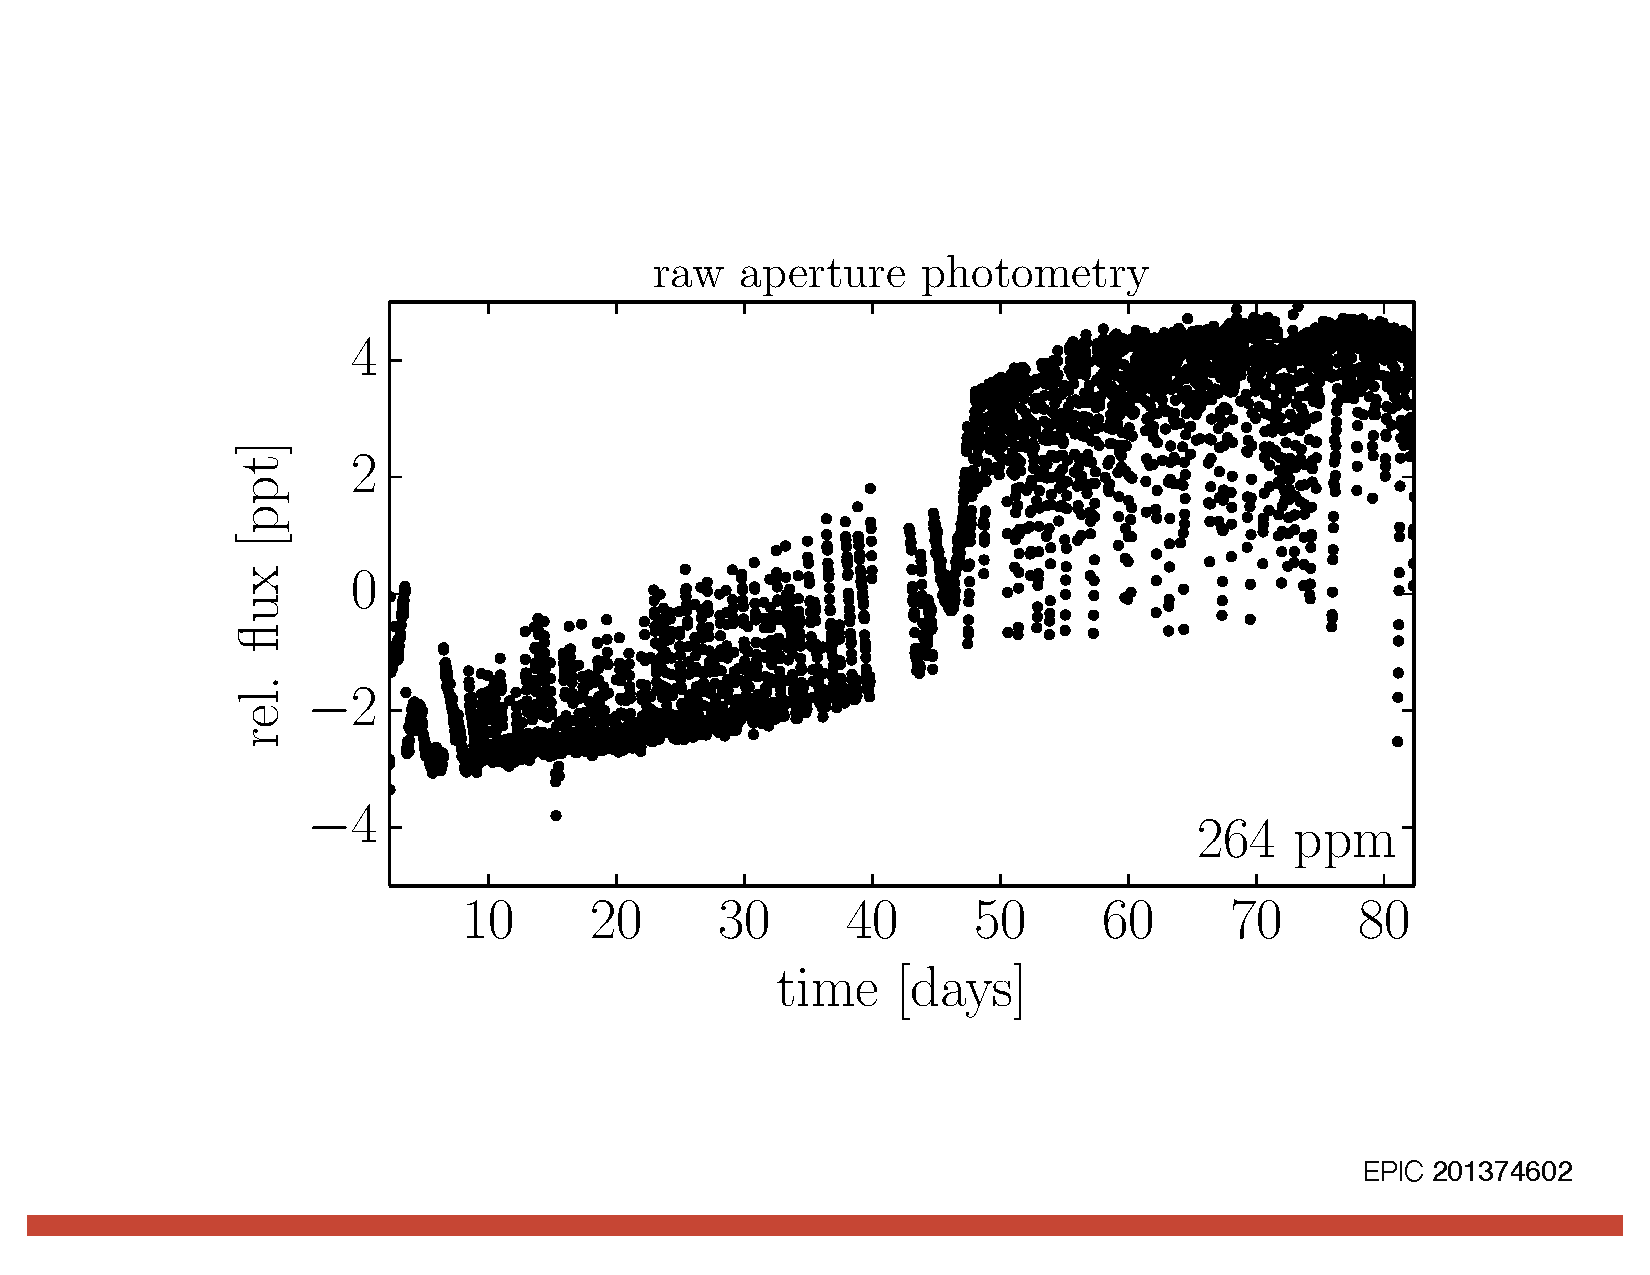
\includegraphics[trim=100 100 100 100, clip, height=\figureheight]{brownbag/brownbagp10.pdf}
\end{frame}

\begin{frame}
  \frametitle{Earth-like transit signals}
  \begin{itemize}
  \item requires good alignment (percent-level)
  \item Earth blocks $10^{-4}$ of the light from the Sun
  \item it does this for 13 hours out of every 365.25 days
  \item the Sun has stochastic variability with an amplitude larger than the signal
  \end{itemize}
\end{frame}

\begin{frame}
  \frametitle{Exoplanet populations {\footnotesize (Foreman-Mackey \etal, arXiv:1406.3020)}}
  ~\hfill
  \includegraphics<1>[height=\figureheight]{1406.3020/results-results.pdf}
  \includegraphics<2>[height=\figureheight]{1406.3020/results-period.pdf}
  \includegraphics<3>[height=\figureheight]{1406.3020/results-radius.pdf}
  \includegraphics<4>[height=\figureheight]{1406.3020/results-rate.pdf}
\end{frame}

\begin{frame}
  \frametitle{Exoplanet populations {\footnotesize (Foreman-Mackey \etal, arXiv:1406.3020)}}
  ~\hfill
  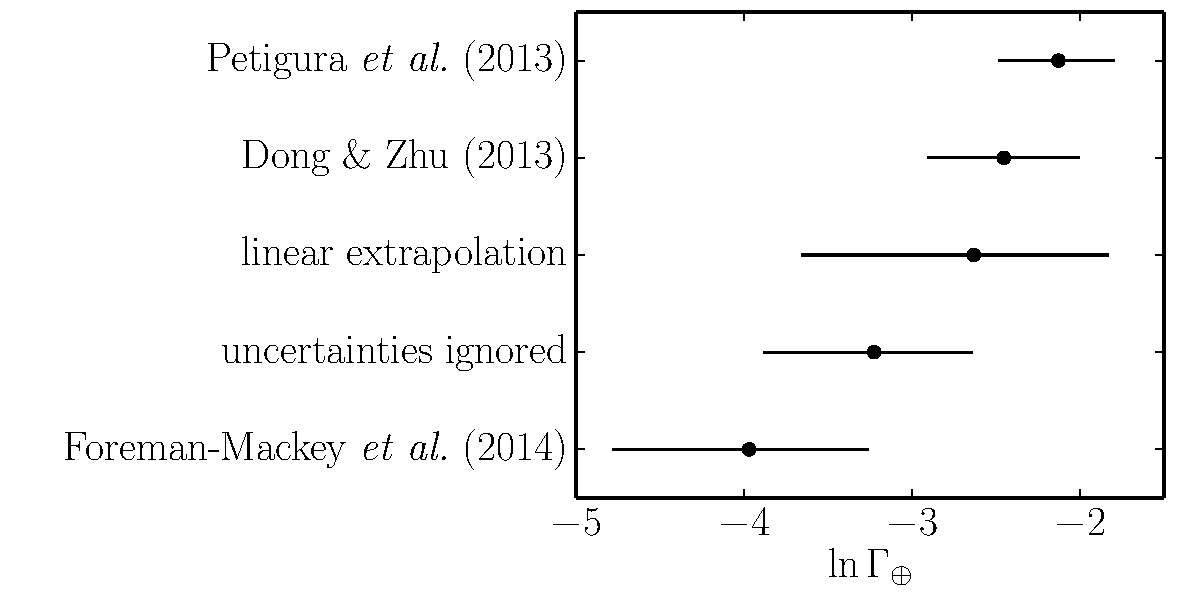
\includegraphics[height=0.75\textheight]{1406.3020/figures-comparison.pdf} \\
  (These results are now superceded by Burke et al 2016.)
\end{frame}

\conclusions

\begin{frame}
  \frametitle{Reminder: $\chi^2$}
  \begin{itemize}
  \item Measures goodness (or badness) of fit.
    \begin{itemize}
    \item (Here $\chi^2$ is a scalar, not a distribution!)
    \item $\chi^2$ is related to the ln of a (Gaussian) likelihood.
    \end{itemize}
  \item It can be written as an inner product (with the noise inverse
    covariance as metric), like a metric squared-distance!
  \end{itemize}
\end{frame}

\begin{frame}
  \frametitle{Reminder: $\chi^2$}
  \begin{eqnarray}
    \chi^2 &\equiv& \sum_i \frac{[y_i - m_i]^2}{\sigma_i^2}
    \nonumber \\
    \chi^2 &=& \transpose{[y - m]}\cdot V^{-1}\cdot [y - m]
    \nonumber \\
    V &=& C
    \nonumber \\
    C_{ij} &\equiv& \sigma_i^2\,\delta_{ij}
    \nonumber \\
    -2\,\ln L &=& \transpose{[y - m]}\cdot V^{-1}\cdot [y - m] + \ln\det V
    \nonumber
  \end{eqnarray}
\end{frame}

\begin{frame}
  \frametitle{Reminder: $\chi^2$}
  \begin{itemize}
  \item $\transpose{[y - m]}\cdot V^{-1}\cdot [y - m] + \ln\det V$
  \item $y$ is your data, $m$ is your model (of an exoplanet signal!).
  \item $V$ encodes your beliefs about your (Gaussian) noise.
  \end{itemize}
\end{frame}

\begin{frame}
  \frametitle{Generalizing (Gaussian) noise}
  \begin{itemize}
  \item Multiple addititive sources of (Gaussian) noise? \emph{Add covariances}.
  \item Adding new components to the noise tensor $V$ is
    equivalent to fitting for new noise processes and marginalizing
    them out.
  \item This is literally as trivial as it sounds.
  \end{itemize}
\end{frame}

\begin{frame}
  \frametitle{Generalizing (Gaussian) noise}
  \begin{eqnarray}
    -2\,\ln L &=& \transpose{[y - m]}\cdot V^{-1}\cdot [y - m] + \ln\det V
    \nonumber \\
    V &=& C + Q
    \nonumber \\
    C_{ij} &\equiv& \sigma_i^2\,\delta_{ij}
    \nonumber \\
    Q &=& \mbox{variance tensor of additional noise}
    \nonumber
  \end{eqnarray}
\end{frame}

\begin{frame}
  \frametitle{Causal idea}
  \begin{itemize}
  \item If a star's behavior can be predicted confidently by
    other stars, then that behavior must be being imprinted by
    the spacecraft.
  \item We are using these ideas to separate spacecraft-induced from
    intrinsic stellar variability {\footnotesize (Wang \etal, arXiv:1508.01853;
    Sch\"olkopf \etal, arXiv:1505.03036)}.
  \end{itemize}
\end{frame}

\begin{frame}
  \frametitle{Data-driven idea}
  \begin{itemize}
  \item The best predictors of a star (or pixel's) behavior are the
    empirical behaviors of \emph{other stars} (or pixels).
  \item The data \emph{are} the model.
  \end{itemize}
\end{frame}

\begin{frame}
  \frametitle{Data-driven idea}
  \begin{itemize}
  \item Imagine that spacecraft pointing is the source of your
    dominant systematic.
  \item Imagine that you have light curves that are good to a part in
    $10^5$, every one of which depends differently on pointing.
  \item The light curves themselves contain the pointing information
    at very high fidelity.
  \item (Much higher fidelity than any measured centroids!)
  \end{itemize}
\end{frame}

\begin{frame}
  \frametitle{Systematic noise model}
  \begin{itemize}
  \item Imagine that we believe that the spacecraft systematics
    (noise) can be modeled as a sum of $M$ basis vectors.
  \item If we can put a Gaussian prior on the linear amplitudes, we
    can fully represent this noise by adding in a rank-$M$ covariance
    matrix.
  \item This is equivalent to fitting and marginalizing!
  \end{itemize}
\end{frame}

\begin{frame}
  \frametitle{Systematic noise model}
  \begin{eqnarray}
    -2\,\ln L &=& \transpose{[y - m]}\cdot V^{-1}\cdot [y - m] + \ln\det V
    \nonumber \\
    V &=& C + B\cdot\Lambda\cdot\transpose{B}
    \nonumber \\
    B &=& \mbox{block of $M$ basis vectors}
    \nonumber \\
    \Lambda &=& \mbox{$M\times M$ prior variance; can $\rightarrow\infty$}
    \nonumber
  \end{eqnarray}
\end{frame}

\begin{frame}
  \frametitle{Systematic noise model}
  \begin{itemize}
  \item $y$ is your data, $m$ is your model (of an exoplanet signal!).
  \item $C + B\cdot\Lambda\cdot\transpose{B}$ encodes your beliefs
    about your (Gaussian) noise, which now has a systematics
    component.
  \end{itemize}
\end{frame}

\begin{frame}
  \frametitle{Systematic noise {\footnotesize (Foreman-Mackey \etal, 1502.04715)}}
  ~\hfill
  \includegraphics<1>[trim=100 100 100 100, clip, height=\figureheight]{brownbag/brownbagp10.pdf}
  \includegraphics<2>[trim=100 100 100 100, clip, height=\figureheight]{brownbag/brownbagp14.pdf}
  \includegraphics<3>[trim=100 100 100 100, clip, height=\figureheight]{brownbag/brownbagp15.pdf}
  \includegraphics<4>[trim=100 100 100 100, clip, height=\figureheight]{brownbag/brownbagp17.pdf}
  \includegraphics<5>[trim=100 100 100 100, clip, height=\figureheight]{brownbag/brownbagp18.pdf}
\end{frame}

\begin{frame}
  \frametitle{Implementation details}
  \begin{itemize}
  \item For expressions like $C + B\cdot\Lambda\cdot\transpose{B}$
    there are matrix inversion and determinant lemmas.
  \item Never use \code{inv()}. Always use \code{solve()}.
  \item Never use \code{det()}. Always use \code{slogdet()}.
  \end{itemize}
\end{frame}

\begin{frame}
  \frametitle{Exoplanet discovery {\footnotesize (Foreman-Mackey \etal, 1502.04715)}}
  ~\hfill
  \includegraphics<1>[height=\figureheight]{1502.04715/figures-corr.pdf}
  \includegraphics<2>[height=\figureheight]{1502.04715/figures-linear.pdf}
  \includegraphics<3>[height=\figureheight]{1502.04715/figures-periodic.pdf}
  \includegraphics<4>[height=\figureheight]{1502.04715/figures-de-trended.pdf}
  \includegraphics<5>[height=\figureheight]{1502.04715/figures-folded.pdf}
  \includegraphics<6>[height=\figureheight]{1502.04715/figures-candidates.pdf}
\end{frame}

\begin{frame}
  \frametitle{Systematic noise model}
  \begin{itemize}
  \item Don't ``fit and subtract'' your systematics!
  \item That isn't conservative.
  \item Signals get distorted {\footnotesize (Foreman-Mackey \etal, 1502.04715)}
  \item You need to marginalize out the noise.
  \item Using $C + B\cdot\Lambda\cdot\transpose{B}$ in $\ln L$ is
    equivalent to fitting the noise simultaneously with your model $m$
    and then marginalizing it out!
  \end{itemize}
\end{frame}

\begin{frame}
  \frametitle{Enormous models}
  \begin{itemize}
  \item Don't be afraid of enormous models.
  \item We sometimes use of order \emph{$10^9$ nuisance parameters} for a
    single \kepler\ lightcurve (70,000 points) {\footnotesize (Wang
      \etal, arXiv:1508.01853)}.
  \item In general, for nuisances, you want to use very flexible
    models but to learn the ``priors''\footnote{They are not really
      priors if you learn them!}.
    \begin{itemize}
    \item \emph{Or} use \emph{train-and-test} frameworks.
    \end{itemize}
  \end{itemize}
\end{frame}

\begin{frame}
  \frametitle{Gaussians are miraculous}
  \begin{itemize}
  \item ~[that is all]
  \end{itemize}
\end{frame}

\begin{frame}
  \frametitle{Stellar variability noise model}
  \begin{itemize}
  \item Imagine that we believe that stars vary stochastically but
    continuously (\ie, with time correlations).
  \item For any model of the amplitude and covariance of the
    variations, we can construct a covariance matrix (to add in).
  \item This is equivalent to fitting and marginalizing!
  \end{itemize}
\end{frame}

\begin{frame}
  \frametitle{Stellar variability noise model}
  \begin{eqnarray}
    -2\,\ln L &=& \transpose{[y - m]}\cdot V^{-1}\cdot [y - m] + \ln\det V
    \nonumber \\
    V &=& C + K
    \nonumber \\
    K_{ij} &=& K(|t_i - t_j|; \theta)
    \nonumber
  \end{eqnarray}
\end{frame}

\begin{frame}
  \frametitle{Gaussian processes}
  ~\hfill
  \includegraphics<1>[height=0.8\figureheight]{george/ind-results.png}
  \includegraphics<2>[height=0.8\figureheight]{george/gp-results.png}
\end{frame}

\begin{frame}
  \frametitle{Implementation details}
  \begin{itemize}
  \item There are many applied-math tricks for making things much
    faster than $N^{2.6}$.
  \item Use \project{george} {\footnotesize (Foreman-Mackey \etal)}.
  \item Marginalizing out the kernel hyperparameters $\theta$ is (in
    general) very expensive.
  \end{itemize}
\end{frame}

\begin{frame}
  \frametitle{Stellar noise model}
  \begin{itemize}
  \item Again, don't ``fit and subtract'' the stellar variability!
  \item Model the variability by adding a Kernel matrix to the covariance matrix.
  \item Again, using $C + K$ in $\ln L$ is equivalent to fitting the
    stochastic variability simultaneously and then marginalizing it
    out!
  \end{itemize}
\end{frame}

\begin{frame}
  \frametitle{Principal limitation 1}
  \begin{itemize}
  \item Assumption of Gaussianity:
    \begin{itemize}
    \item outliers are death
    \item variabilities are all skew
    \item multiplicative noise?
    \end{itemize}
  \item Generalizaions are \emph{intractable} or evil.
    \begin{itemize}
    \item dictionary methods, other processes
    \item the copula
    \end{itemize}
  \end{itemize}
\end{frame}

\begin{frame}
  \frametitle{Principal limitation 2}
  \begin{itemize}
  \item Heuristic decisions
    \begin{itemize}
    \item model complexity
    \item prior forms and hyper-parameters
    \item detection thresholds
    \end{itemize}
  \end{itemize}
\end{frame}

\conclusions

\end{document}
